\section{Infraestrutura}

    Quanto a infraestrutura será necessário um 
    investimento para possibilitar o monitoramento
    e garantir a segurança do sistema.

    Para ser possível verificar a temperatura atual do 
    freezer obviamente será imprescindível um termômetro,
    para ser mais especifico um sensor como uma sonda para facilitar
    o processo de instalação, que será integrado
    a um microcontrolador, como um CLP ou arduíno, 
    como mostrado na figura \ref{fig:termometro}.

    Para a escolha do termômetro o critério usado foi 
    a variação de temperatura, como especificado na demanda
    ``vacinas que devem ser conservadas a uma temperatura entre 2º à 8º C.''
    \citeonline{senaiDemanda},
    dito isso, como a variação de temperatura é pequena se faz 
    importante que o sensor tenha uma boa precisão ao 
    invés de suportar uma grande variação de temperatura.

    \begin{figure}[h]
        \caption{Sensor de temperatura}
        \centering
        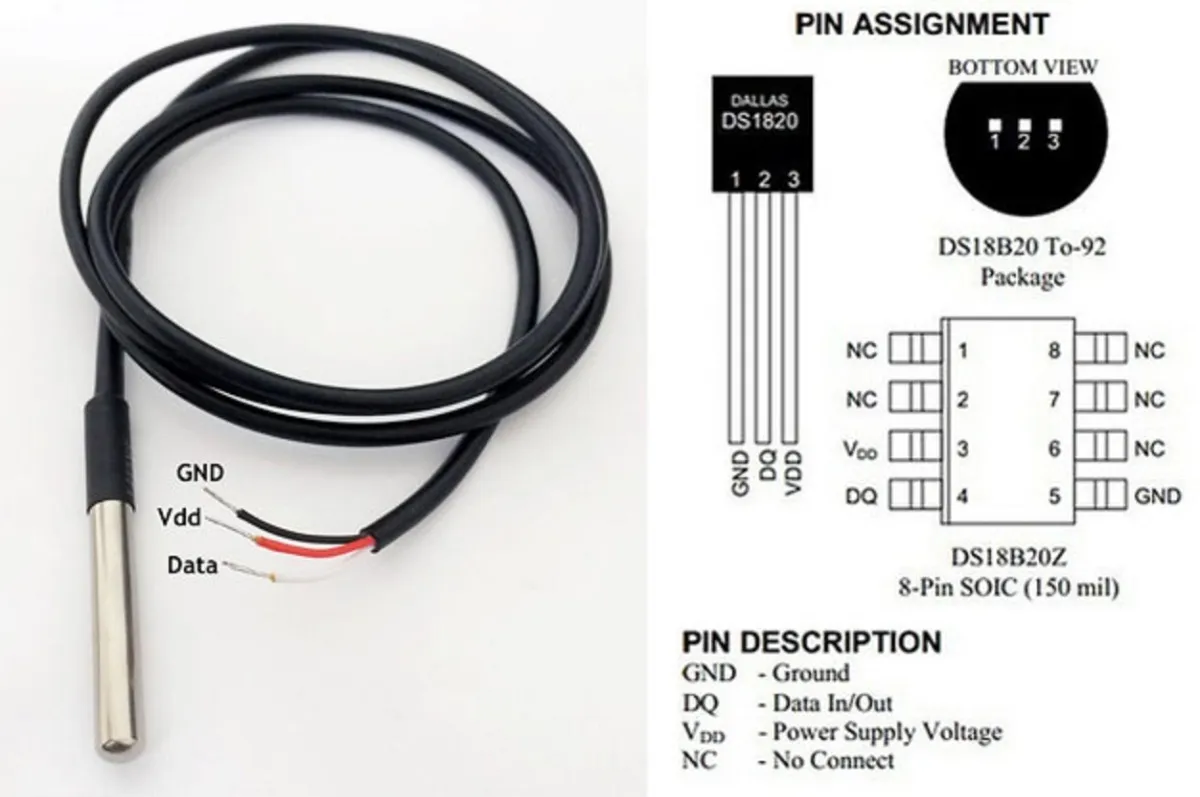
\includegraphics[width=0.8\textwidth]{img/termometro_esquema.png}
        \legend{Fonte: Retirado do site Mercado Livre \protect\footnotemark}
        \label{fig:termometro}
    \end{figure}

    \footnotetext{
        Disponível em: \url{https://produto.mercadolivre.com.br/MLB-1685461701}.
        Acesso em: 14 dez. 2020
    }

    Como o sensor térmico precisa ser ligado a um microcontrolador
    para poder transmitir a um servidor, pensando na segurança e 
    confiabilidade do sistema cada freezer deve ter seu próprio 
    microcontrolador para que na ocorrência de algum imprevisto
    isso possa ser facilmente isolado e corrigido sem afetar 
    outras partes do sistema.

    Considerando que cada freezer terá seu próprio microcontrolador
    facilitará assim a compra da peça pois cada microcontrolador 
    terá apenas a entrada do termômetro e do sensor de porta aberta;
    como saída um modulo de internet, uma lampada e uma sirene, 
    devido a esta quantidade de entradas e saídas pequena o custo
    de cada microcontrolador pode cair consideravelmente.

    \begin{figure}[ht]
        \caption{Arduíno Uno}
        \centering
        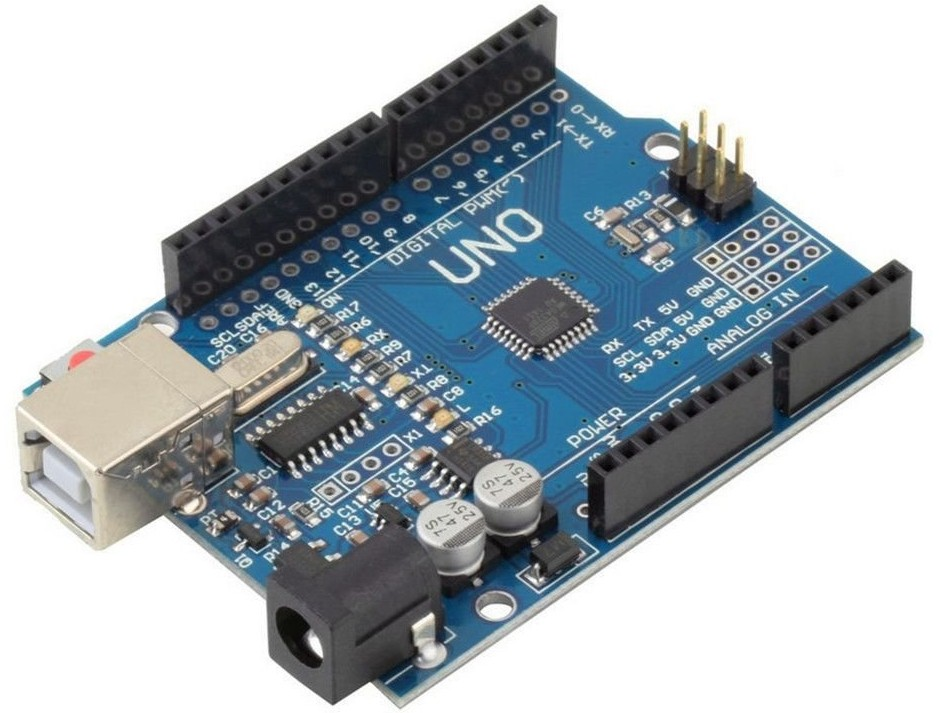
\includegraphics[width=0.85\textwidth]{img/arduino_uno.jpg}
        \legend{Fonte: Imagem retirada do site Eletrogate
            \protect\footnotemark
        }
        \label{fig:arduinoUno}
    \end{figure}

    \footnotetext{
        Disponível em: \url{https://www.eletrogate.com/uno-r3-smd-ch340-cabo-usb-para-arduino}.
        \\
        Acessado em 15 de Dez. 2020
    }

    Assim como mostrado na figura \ref{fig:arduinoUno}
    o microcontrolador escolhido é o arduíno Uno
    por ser simples, rápido, pequeno e de um baixo custo,
    este é muito usado em automação de processos
    de vários tipos. È recomendável para manter o 
    arduíno conservado e funcional coloca-lo em um case
    \footnote{
        Exemplo de case: \url{https://www.eletrogate.com/case-para-arduino-uno-em-acrilico-transparente}
        Acessado em 15 de Dez. 2020
    },
    uma caixa feita normalmente de plástico ou acrílico 
    para guardar e conservar-lo.

    Quanto ao servidor apesar de ser uma parte importante 
    da infraestrutura, pensando em manter a simplicidade 
    e segurança do sistema optamos por uma nuvem privada,
    como o Azure, AWS ou Google Cloud, no qual todos os 
    dados e infraestrutura é de responsabilidade da 
    nuvem contratada, sendo necessário investir apenas 
    em um bom link de internet para acessar os recursos 
    da nuvem.

    Sobre o link de internet para garantir a 
    alta disponibilidade do sistema tanto 
    para transmitir os dados dos sensores 
    como para visualizar e se manter atualizado
    no sistema web deve-se colocar um link redundante,
    assim a empresa não ficará presa a um único provedor 
    e em caso de alguma eventual falha o segundo link 
    assumirá mantendo tudo em funcionamento.
